Что делать, если мы хотим классифицировать объекты не на два класса, а на большее количество? Есть два разных подхода

\textbf{One vs Rest}

Исходя из названия понятен смысл: мы берём один класс, все остальные объекты помечаем другим классом.
Далее на этом тренируем классификатор, потом берём следующий класс, кроме этого второго класса, помечаем
остальные объекты противоположным классом. И так тренируем столько классификаторов, сколько у нас есть
классов.

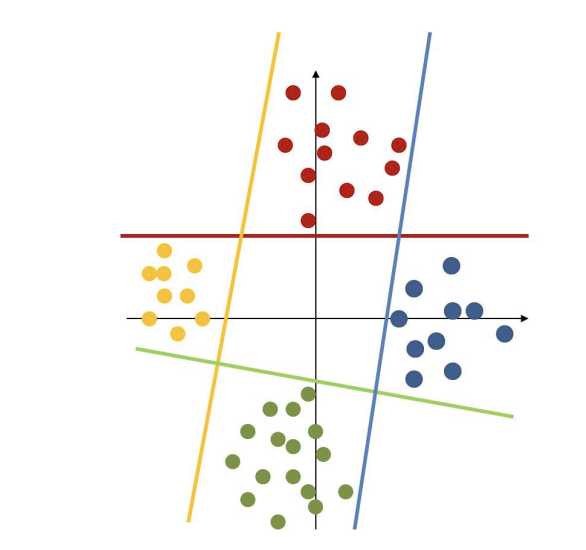
\includegraphics{images/10_1.png}

Довольно очевидно, что тот, у кого наибольшая вероятность в таком процессе, предсказывается следующим
образом: берётся точка в пространстве, мерим вероятности относительно каждого из построенных классификаторов и смотрим у кого больше вероятность, к тому классу мы и относим. Как должны быть расположены
классы в пространстве признаков, чтобы поломать такой классификатор?
Центры каждого класса должны быть расположены на одной прямой, такая ситуация поломает подобную
классификацию.
Понятно, что крайние два класса будут хорошо разделяться, а средний не будет отделяться вообще никак,
потому что нельзя линейным классификатором (одной гиперплоскостью) отделиться от двух других классов
справа и слева.

Есть ещё одна проблема, которая менее заметна на первый взгляд: серые зоны. На рисунке серую зону
можно увидеть в центре. Если в ту область попадают объекты из обучающей выборки, непонятно к какому
классу их отнести, у нас нет таких данных. Равно как и в остальных серых зонах по бокам, тоже непонятно
что будет происходить. В достаточно простом случае мы можем это предсказать - финальное решение поделит
серые зоны между каждыми двумя классификаторами пополам, а в центре на столько частей сколько классов
всего. Несовпадение границ проведенных и границ финальных связано с тем, что мы принимаем решение
коллективно.

\textbf{One vs One}

В такой стратегии мы будем сравнивать один класс с каким-нибудь другим классом из имеющихся, применяя
опять линейный классификатор. 

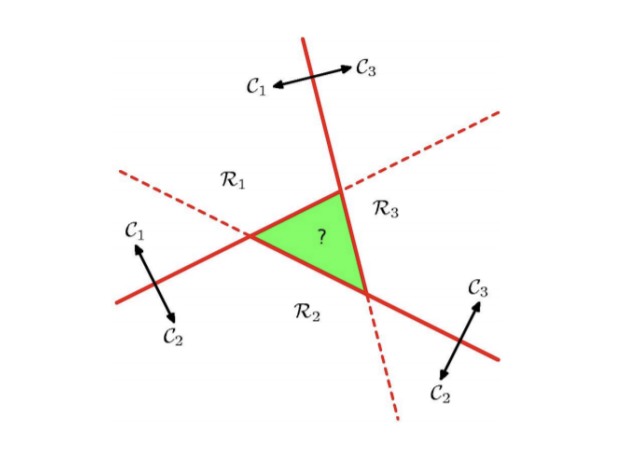
\includegraphics{images/10_2.png}

Буквами $R_i$ на картинке обозначены кластера тех объектов, которые мы будем классифицировать. А сплошные линии, переходящие в пунктирные это классификаторы. Класс $c_2$
отделяется классификатором от класса $c_1$, не смотря совершенно на класс 3, и тд.

\textbf{Сравнение}

В одном случае мы тренируем только $k$ классификаторов, но тренируем их на полном датасете каждый --- это отражается на времени обучения всего классификатора. Во втором случае
мы тренируем квадратичное число классификаторов, но с другой стороны у нас есть плюс в том, что если
классы равномерно распределены, то каждый раз мы будем только два кластера из всех рассчитывать (то
есть меньше чем весь датасет). Но в стратегии one vs one есть проблема в том, что слишком мало сэмплов. То
есть существуют классы, которых меньше в выборке, и с ними может возникнуть проблема.
Надо заметить, что в таком процессе one vs one мы убираем строки из матрицы признаков, а не столбцы, то
есть количество признаков сохраняется, а именно количество объектов при обучении уменьшается.